\section*{Introduction}
In this report the goal was to implement and analysis of Dissipative Particle Dynamics (DPD) simulations in 2D. DPD is a mesoscopic simulation method that bridges the gap between microscopic methods like Molecular Dynamics and macroscopic methods like Computational Fluid Dynamics. In DPD, particles represent clusters of molecules rather than individual atoms, allowing for simulation of larger systems and longer time scales.
The simulation implements three types of forces between particles:
\begin{enumerate}
	\item Conservative forces (soft repulsion)
	\item Dissipative forces (friction-like)
	\item Random forces (thermal fluctuations)
\end{enumerate}
These forces combine to create a thermostat that maintains the system temperature while preserving hydrodynamic behavior.
The simulation was implemented in Python, for further information regarding the keycomponents of the implementation consult the README.md file.
% \subsection{Methodology}
% The simulation was implemented in Python with the following key components:
% \begin{enumerate}
% 	\item \textit{Numerical Integration}: A velocity-Verlet scheme was implemented to integrate the equation of motion.
% 	\item \textit{Force Calculation}: The three DPD forces were implemented as follows:
% 		\item
% 	\item \textit{Molecular Structures}:
% 	\item \textit{Cell List Algorithm}:
% 	\item \textit{Periodic Boundary Conditions}
% 	\item \textit{Wall Implementation:}
% \end{enumerate}
% For all simulations, the following base parameters were used
% \begin{itemize}
% 	\item Box size: $L = 15.0$
% 	\item Particle density: $\rho  = 4.0$ (total $N = 900$ particles)
% 	\item Cutoff radius: $r_c = 1.0$
% 	\item Dissipative coefficient: $\gamma = 4.5$
% 	\item Random force coefficient: $\sigma = 1.0$
% 	\item Bond spring constant: $K_S = 100.0$
% \end{itemize}
\section{Test Simulation}
For the preliminary test, a system containing only fluid particles was simulated with conservative force coefficient $a_{ij} = 25$ using various timestep over $1000$ steps.
\begin{figure}[H]
	\begin{center}
		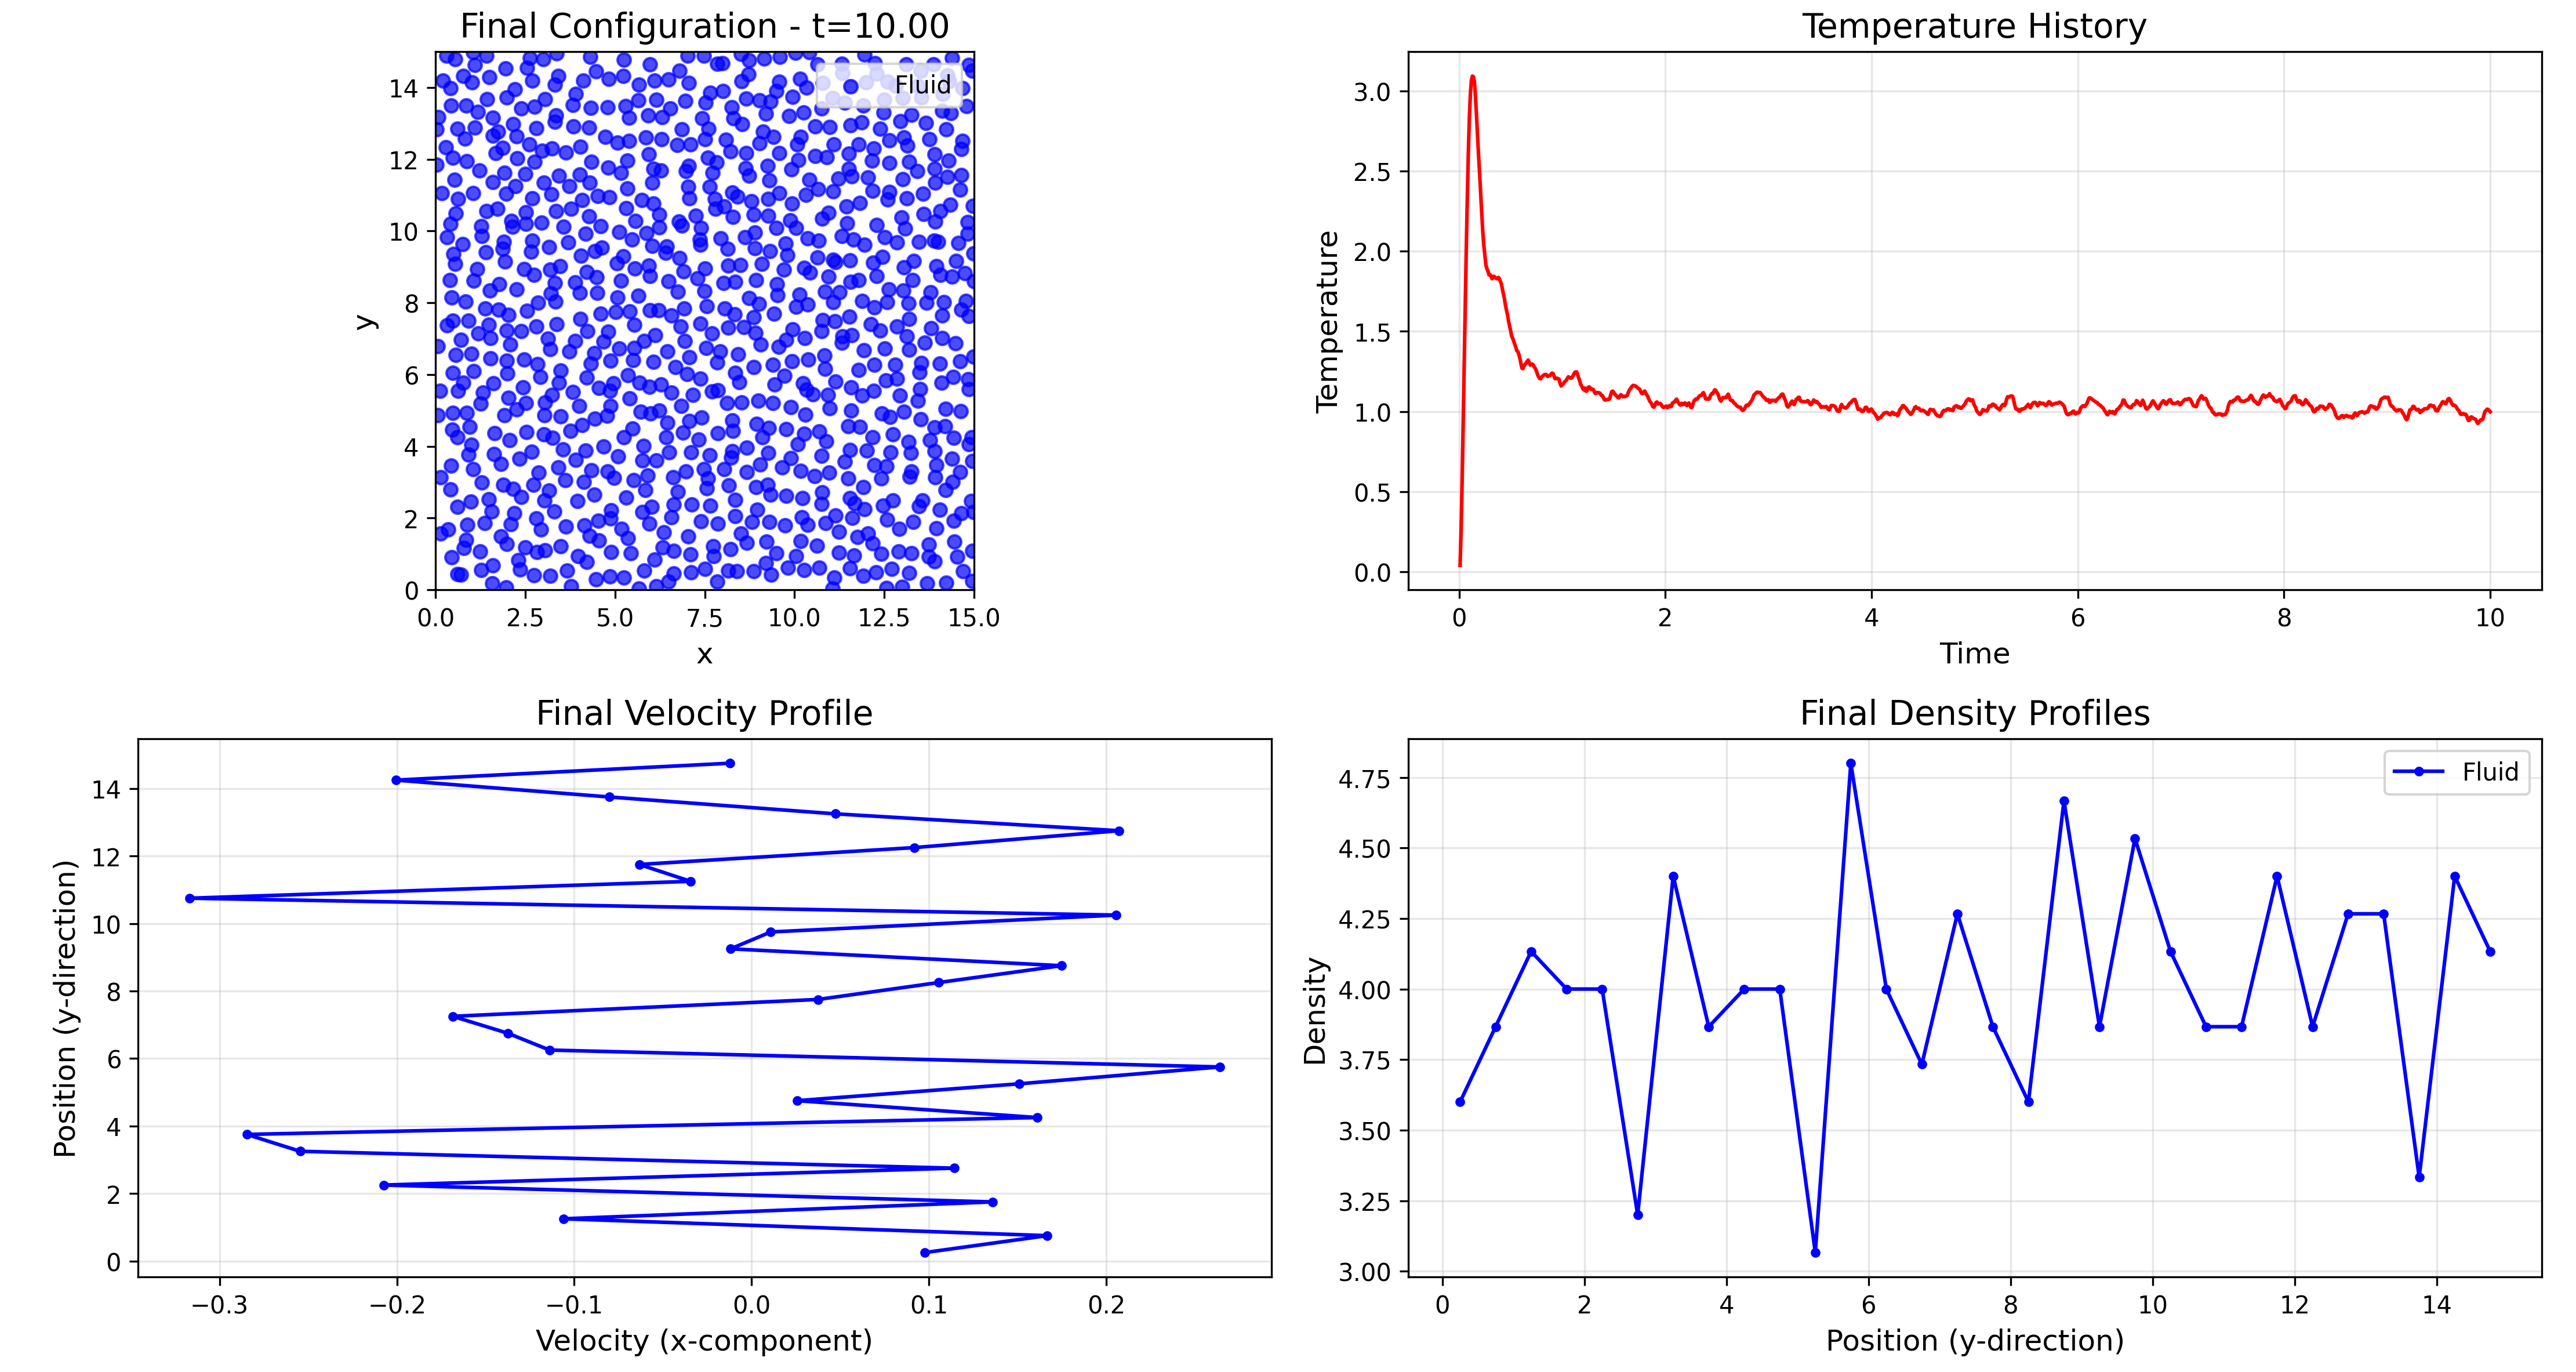
\includegraphics[width=0.95\textwidth]{figures/test_final_vis.png}
	\end{center}
	\caption{Test Scenario with $dt = 0.01$ and $1000$ steps}\label{fig:test}
\end{figure}
\subsection{Temperature Stability}
As shown in Figure \ref{fig:test}, the temperature initially spiked but quickly stabilized around $1.0$, which is the desired temperature set by the DPD thermostat parameters. This confirms proper implementation of the dissipative and random forces.
\subsection{Conservation of Momentum}
Total momentum was being tracked throughout the simulation and remained constant with only minor numerical fluctuations, confirming the correct implementation of the forces.
\subsection{Timestep Dependency}
Multiple test runs were performed using different timestep values. For $dt = 0.01$, the system showed good stability while having reasonable computational efficiency. Larger timesteps led to instabilities, while smaller timesteps significantly increased computation time without relevant accuracy improvements. 

